\documentclass[11pt]{beamer}
\usetheme{Boadilla}
\usepackage[utf8]{inputenc}
\usepackage[french]{babel}
\usepackage[T1]{fontenc}
\usepackage{amsmath}
\usepackage{amsfonts}
\usepackage{amssymb}
\usepackage{graphicx}
%\usepackage{movie15}
\usepackage{media9}
\author[Acier, Barret, Reisser, Vanel]{Valérian Acier, Nelly Barret, Juliette Reisser, Guillaume Vanel}
\title[PIC]{Projet PIC \\ Piano Intelligent Connecté}
%\setbeamercovered{transparent} 
\setbeamertemplate{navigation symbols}{} 
%\logo{} 
%\institute{} 
\date{29 janvier 2020} 
%\subject{} 
\begin{document}

\begin{frame}
\titlepage
\end{frame}

%\begin{frame}
%\tableofcontents
%\end{frame}

%\begin{frame}{Contexte et motivations}
%Contexte
%\begin{itemize}
%    \item Objet connecté intelligent
%    \item Arduino, leds, boutons et fils
%\end{itemize}
%~\\
%Motivations
%\begin{itemize}
%    \item Réception d'un morceau musical créé par l'utilisateur
%    \item Création de la suite du morceau musical
%    \item Mise en place d'une interface entre l'utilisateur, l'arduino et le serveur
%\end{itemize}

%\end{frame}

%\begin{frame}{Frame Title}
%\includemovie{1cm}{1cm}{architecture_pic.gif}
%\includemedia[width=0.6\linewidth,height=0.6\linewidth,activate=pageopen, passcontext, transparent, addresource=architecture_pic.gif, flashvars={source=architecture_pic.gif}]{\includegraphics[width=0.6\linewidth]{penguins}}{VPlayer.swf}
%\end{frame}

%\begin{frame}{Résumé} % Contexte et motivations
%\begin{center}
%    Piano connecté capable de produire la suite d'une mélodie jouée
%\end{center}
%\end{frame}

\begin{frame}{Scénarios}
\begin{itemize}
    \item Alice, lycéenne et passionnée de piano
\end{itemize}
Alice est une jeune lycéenne et se passionne pour le piano. Elle aimerait créer ses propres compositions mais n'a pas assez d'inspiration pour créer un morceau complet. Elle utilise donc PIC après avoir créé une petite mélodie pour s'inspirer de ce que PIC va produire pour créer la suite de sa composition.\\~\\

\begin{itemize}
    \item Bob, enseignant-chercheur en IA
\end{itemize}
Bob est enseignant-checheur en Intelligence Artificielle. Il travaille sur un projet dont le but est de prédire la suite d'une composition musicale au piano. Il a développé et implémenté un algorithme capable de créer la suite d'une séquence musicale. Il souhaite le tester et utilise PIC. Ainsi il peut tester différentes mélodies. 
    
\end{frame}

\begin{frame}{Configuration matérielle}
\begin{itemize}
    \item 1 carte Arduino
    \item 6 boutons (capteurs)
    \item 6 LEDs (actionneurs)
\end{itemize}
\end{frame}


\begin{frame}{Technologies logicielles}
Magenta
\begin{itemize}
    \item Librairie Python open-source (TensorFlow) 
    \item Manipulation de sources de données musicales et picturales
    \item Mise à disposition de modèles de Machine Learning
    \item Génération de contenu grâce à ces modèles
\end{itemize}
~\\
\begin{center}
    
\includegraphics[scale=0.05]{logo-magenta.png}
\end{center}
    
\end{frame}

\begin{frame}{Architecture}
Étapes :
\begin{itemize}
    \item Réception de la mélodie via les boutons
    \item Envoi au serveur
    \item Traitement sur le serveur (Magenta)
    \item Renvoi aux clients et au PIC
\end{itemize}
\begin{center}
    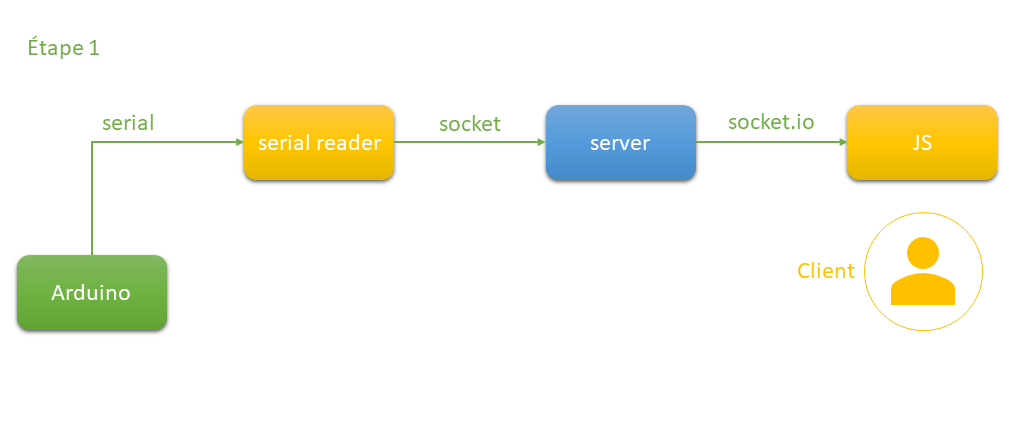
\includegraphics[scale=0.23]{etape1.png}
    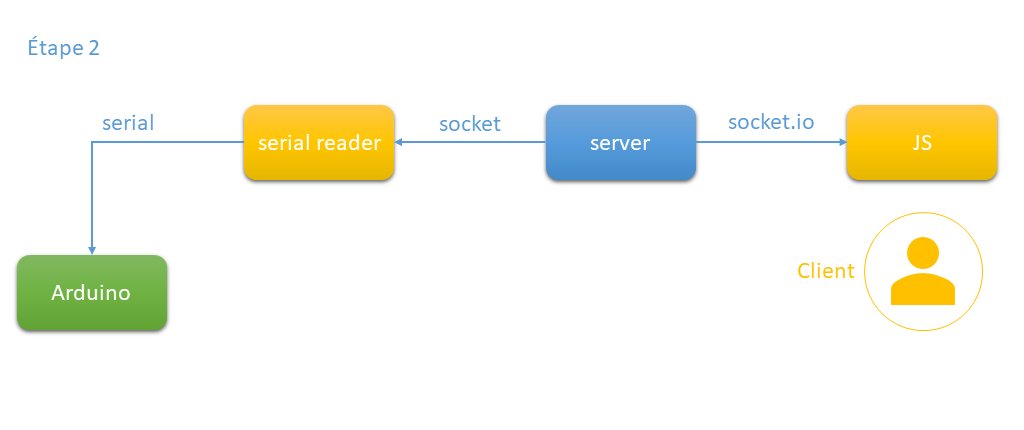
\includegraphics[scale=0.23]{etape2.png}
\end{center}
\end{frame}


\begin{frame}{Intelligence ajoutée}
\begin{itemize}
    \item Complétion du morceau commencé à partir des capteurs
    \item Restitution via les actionneurs
    \item 
\end{itemize}
\end{frame}

\begin{frame}{Conclusion}
\begin{itemize}
    \item Utilisation de l'arduino comme support pour un objet intelligent et connecté
    \item Utilisation de capteurs et d'actionneurs
    \item Communication entre l'arduino et le serveur
\end{itemize}
\end{frame}
\end{document}